\documentclass[12pt,letterpaper]{article}


\newcommand{\studentname}{Ben Bassett}
\newcommand{\labpartner}{Katrina Sumarli}

\title{\textsc{Lab 02: Harmonic Oscillator with Air Drag}}
\newcommand{\shorttitle}{Harmonic Oscillator with Drag}

\newcommand{\course}{PHY310}
\newcommand{\labdate}{09-10-2024}

%------------------------------------------------------------------------------------------------------------

\usepackage[letterpaper,left=1in,right=1in,bottom=1in,top=1in]{geometry}
\usepackage{fancyhdr}
\usepackage{subfigure}
\usepackage{graphicx}
\usepackage{amsmath}
\usepackage{cleveref}
\usepackage{booktabs}
\usepackage[british]{babel}
\usepackage[square,comma,numbers,sort&compress]{natbib}
\usepackage{csvsimple}
\usepackage{graphicx}
\usepackage{pgfplotstable}
\usepackage{textcomp,gensymb}
\usepackage{array}
\usepackage{tabu}
\usepackage{multirow}
\usepackage{url}
\usepackage{lipsum}
\pgfplotsset{compat=1.9}% supress warning
\begin{document}

%------------------------------------------------------------------------------------------------------------

\setlength{\parindent}{1em}
\setlength{\parskip}{0.5em}
\author{\course~Lab Journal \\ \\ \studentname\,\& \labpartner}
\date{\labdate}

\renewcommand\abstractname{Summary}

\pagestyle{fancy}
\fancyhead{}
\fancyhead[l]{\course:~\shorttitle}
\fancyhead[r]{\studentname}
\fancyfoot{}
\fancyfoot[C]{\thepage}
\renewcommand{\headrulewidth}{0pt}
\renewcommand{\footrulewidth}{0pt}

\renewcommand\bibname{References}

%------------------------------------------------------------------------------------------------------------

\renewcommand\abstractname{Abstract}
\maketitle

% COMMENT IN IF ASKED TO SUBMIT REPORT WITH ABSTRACT
%\begin{abstract}
%Maximum 200 words.
%\end{abstract}

\section{Purpose}
This lab aimed to measure the coefficient of air drag as a function of cross-sectional area.

\section{Experimental Apparatus}

We were given a metal spring, cardstock paper, weights, string, scissors, a (drawing) compass, and a retort stand with a horizontal clamp. Our general setup is illustrated in Figure \ref{fig:setup}.

 \begin{figure}[h]
     \centering
     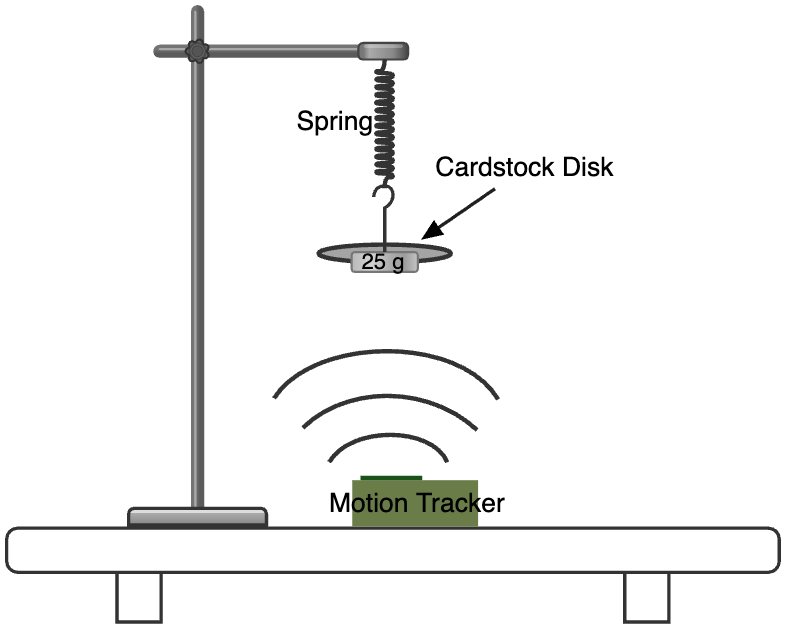
\includegraphics[width=4in]{images/setup.png}
     \caption{A diagram of our experimental setup}
     \label{fig:setup}
 \end{figure}

% \pagebreak
\section{Procedure}

 We used the compass and scissors to cut out four (4) circles of 4 cm, 6 cm, 8 cm, and 10 cm. We hung the spring vertically on the horizontal retort clamp, and measured it's equilibrium position. Then we attached the weight hanger (5 g) and placed 40 g of weight on it. We then measured the new equilibrium position. Then we reduced the total weight on the spring to 25 g to capture more exaggerated data, placed the motion sensor beneath, and did 5 30-second motion recordings. The first one had only the 25 g, but the second had the 4cm disk, the third the 6 cm disk, the fourth the 8cm disk, and the fifth the 10 cm disk. On each run, we held the spring as far up as possible, so that the spring was at it's 0 g equilibrium position. We then began recording and released it.

\section{Results}

First, we attempted to get a measurement of the spring constant. To do this, we measured the displacement of the spring's equilibrium at 45 g to be $23.4$ cm $=0.234$ m. Let's derive how to find $k$:

\begin{align*}
    \sum F&=ma = 0 \\
    F_S-F_G&=ma = 0 \\
    -k\Delta x+mg&=ma = 0 \\
    k\Delta x&=mg
\end{align*}
\begin{equation}
    k=\frac{mg}{\Delta x}
\end{equation}

Let's substitute in our numbers:

\begin{equation*}
    k=\frac{0.045 \text{ kg} \times 9.81 \frac{\text{m}}{\text{s}^2}}{0.234 \text{ m}} = \mathbf{1.9} \frac{\textbf{kg}}{\textbf{s}^\mathbf{2}}
\end{equation*}

After collecting our data on the Labquest, we exported the 5 runs as a single text file with time, position, velocity, and acceleration. I then used a Python program (see \url{https://github.com/benonymity/PHY-310/blob/main/Lab2/analysis.py}) to analyze and graph the data. First, it imports all data from the text file, then separates each run. For each run, it averages all the data to normalize it around a center line for graphing (which should be the equilibrium position), finds the absolute value of each maximum and minimum, and fits those points to two curves; one described by the equation
\begin{equation}
    y=Ae^{-bt} + C
\label{eqn:envelope}
\end{equation}
Which is simply the envelope, or the damping term of the oscillation. It also fit the data to the ideal curve for the entire oscillation, represented by
\begin{equation}
    y=Ae^{-bt} \cos \left(\omega t + \phi\right) + C
\label{eqn:oscillation}
\end{equation}
This is derived from the analysis of the drag force 
\begin{equation}
    \label{eqn:drag}
    F_D=3\pi \mu Dv
\end{equation}
We use differential analysis to get the equation of motion for dampened harmonic oscillation, which in it's full form is
\begin{equation}
    y=Ae^{-\frac{b}{2m}t} \cos \left(\sqrt{\frac{k}{m} - \frac{b^2}{4m^2}} t + \phi\right)
\end{equation}
However, we can solve $\omega$ and $b$ (which is really something like $3\pi \mu D$) as simple constants.

After fitting the curves, we got 5 equations, whose constants are recorded in the two tables. Table \ref{tab:envelope} has all of the constants for the curve fit to the envelope equation (Equation \ref{eqn:envelope}), while Table \ref{tab:oscillation} is from the curve fit to the entire oscillatory equation (Equation \ref{eqn:oscillation}). The difference between the two is often significant, which raises some questions. However, this is likely due to the inconsistency in peaks vs the consistency of the entirety of the curve. For instance, Figure \ref{fig:4cm} has two strange spikes on it's peaks, and since the peaks are far more heavily weighted in the envelope equation vs. the oscillation one, such anomalies are less weighted. Our experimental setup was also imperfect, as we have no guarantee that some of the energy of the spring was going into $x$ shifts, as we couldn't lock the spring in into the $y$ direction. Also, doing this experiment in a lab of moving, breathing, speaking humans doubtlessly introduced air currents which resulted in minute changes when the oscillations became extremely small, such as when a disk 10 cm in radius was oscillating in millimeters. Stable movement in such an unpredictable environment is hard to expect.

Analyzing these constants to find a relationship between damping constant and cross-sectional area requires us to make b independent of mass, as each time we change out the cardstock disk, there is a subtle change in mass on the spring. To do this, we'll multiply each of our fitted $b$ values by $2m$ to remove that changing variable and isolate $b$ as it changes with area. See Table \ref{tab:barea}.

After isolating $b$ with respect to area, we graph it as shown in Figure \ref{fig:benv} and Figure \ref{fig:bosc}, which shows us that there is a linear relationship of $b$ and area. Increase the cross-sectional area, and $b$ will increase linearly with it, prefixed by some constant slope ($\approx3\pi\mu$).

\section{Error}

All of the values in the tables are precise to more decimal points than our data was in (mm), but this is so we can carry those computed values through and round to significant digits at the end. All of the mass measurements were done on a scale that is $± 0.01$ g, and all of the motion sensor measurements were $± 1$ mm. We didn't do much actual math to these original values, but our error propagation still needs to be done. I used Python to calculate the standard deviation of all our values, which came out to be $0.038029$ m. We use the error propagation formula
\begin{equation}
    \delta f=\sum_i \left(\frac{\delta f}{\delta a_i}\right)\delta a_i^2
\end{equation}
So we'll square $0.038029$ m to end up with a final error of $± \mathbf{0.001446204841}$ m.

\section{Conclusions}

We observed a linear relationship between our circular cutouts (chosen so that their area could be easily measured, and to ensure uniform air flow, where something with sharp corners seems like it would introduce more turbulent flow.) This fits with our knowledge of Stoke's Law (Equation \ref{eqn:drag}), and shows us that increasing our surface area linearly increases our drag.

\begin{table}[ht]
\centering
\begin{tabular}{llllllll}
                                & Area                            & Mass                         & $A$                          & $b$                          & $C$                          & $\omega$                     & $\phi$                        \\ \cline{2-8} 
\multicolumn{1}{l|}{No Disk}    & \multicolumn{1}{l|}{13 cm$^2$}  & \multicolumn{1}{l|}{25.00 g} & \multicolumn{1}{l|}{0.10168} & \multicolumn{1}{l|}{0.01699} & \multicolumn{1}{l|}{0.00017} & \multicolumn{1}{l|}{7.84299} & \multicolumn{1}{l|}{0.65649}  \\ \cline{2-8} 
\multicolumn{1}{l|}{4 cm Disk}  & \multicolumn{1}{l|}{50 cm$^2$}  & \multicolumn{1}{l|}{25.99g}  & \multicolumn{1}{l|}{0.11307} & \multicolumn{1}{l|}{0.05288} & \multicolumn{1}{l|}{0.00016} & \multicolumn{1}{l|}{7.66648} & \multicolumn{1}{l|}{–1.81840} \\ \cline{2-8} 
\multicolumn{1}{l|}{6 cm Disk}  & \multicolumn{1}{l|}{113 cm$^2$} & \multicolumn{1}{l|}{27.43 g} & \multicolumn{1}{l|}{0.11154} & \multicolumn{1}{l|}{0.12032} & \multicolumn{1}{l|}{0.00049} & \multicolumn{1}{l|}{7.39021} & \multicolumn{1}{l|}{–2.23723} \\ \cline{2-8} 
\multicolumn{1}{l|}{8 cm Disk}  & \multicolumn{1}{l|}{201 cm$^2$} & \multicolumn{1}{l|}{28.95 g} & \multicolumn{1}{l|}{0.12103} & \multicolumn{1}{l|}{0.19301} & \multicolumn{1}{l|}{0.00030} & \multicolumn{1}{l|}{7.12469} & \multicolumn{1}{l|}{–1.85440} \\ \cline{2-8} 
\multicolumn{1}{l|}{10 cm Disk} & \multicolumn{1}{l|}{314 cm$^2$} & \multicolumn{1}{l|}{31.32 g} & \multicolumn{1}{l|}{0.14428} & \multicolumn{1}{l|}{0.31610} & \multicolumn{1}{l|}{0.00050} & \multicolumn{1}{l|}{6.69661} & \multicolumn{1}{l|}{–2.01379} \\ \cline{2-8} 
\end{tabular}
\caption{Constants in Oscillation Fit}
\label{tab:oscillation}
\end{table}

\begin{table}[ht]
\centering
\begin{tabular}{llllll}
                                & Area                            & Mass                         & $A$                          & $b$                          & $C$                          \\ \cline{2-6} 
\multicolumn{1}{l|}{No Disk}    & \multicolumn{1}{l|}{13 cm$^2$}  & \multicolumn{1}{l|}{25.00 g} & \multicolumn{1}{l|}{0.10170} & \multicolumn{1}{l|}{0.01695} & \multicolumn{1}{l|}{0.03657} \\ \cline{2-6} 
\multicolumn{1}{l|}{4 cm Disk}  & \multicolumn{1}{l|}{50 cm$^2$}  & \multicolumn{1}{l|}{25.99g}  & \multicolumn{1}{l|}{0.10584} & \multicolumn{1}{l|}{0.06679} & \multicolumn{1}{l|}{0.01263} \\ \cline{2-6} 
\multicolumn{1}{l|}{6 cm Disk}  & \multicolumn{1}{l|}{113 cm$^2$} & \multicolumn{1}{l|}{27.43 g} & \multicolumn{1}{l|}{0.11132} & \multicolumn{1}{l|}{0.17353} & \multicolumn{1}{l|}{0.00989} \\ \cline{2-6} 
\multicolumn{1}{l|}{8 cm Disk}  & \multicolumn{1}{l|}{201 cm$^2$} & \multicolumn{1}{l|}{28.95 g} & \multicolumn{1}{l|}{0.12131} & \multicolumn{1}{l|}{0.27732} & \multicolumn{1}{l|}{0.00495} \\ \cline{2-6} 
\multicolumn{1}{l|}{10 cm Disk} & \multicolumn{1}{l|}{314 cm$^2$} & \multicolumn{1}{l|}{31.32 g} & \multicolumn{1}{l|}{0.15710} & \multicolumn{1}{l|}{0.45115} & \multicolumn{1}{l|}{0.00571} \\ \cline{2-6} 
\end{tabular}
\caption{Constants in Envelope Fit}
\label{tab:envelope}
\end{table}

\begin{table}[ht]
\centering
\begin{tabular}{lllll}
                                & Area                            & Mass                         & Oscillation $b\times 2m$ & Envelope $b\times 2m$ \\ \cline{2-5} 
\multicolumn{1}{l|}{No Disk}    & \multicolumn{1}{l|}{13 cm$^2$}  & \multicolumn{1}{l|}{25.00 g} & \multicolumn{1}{l|}{0.4248}             & \multicolumn{1}{l|}{0.4238}          \\ \cline{2-5} 
\multicolumn{1}{l|}{4 cm Disk}  & \multicolumn{1}{l|}{50 cm$^2$}  & \multicolumn{1}{l|}{25.99g}  & \multicolumn{1}{l|}{1.374}              & \multicolumn{1}{l|}{1.736}           \\ \cline{2-5} 
\multicolumn{1}{l|}{6 cm Disk}  & \multicolumn{1}{l|}{113 cm$^2$} & \multicolumn{1}{l|}{27.43 g} & \multicolumn{1}{l|}{3.300}              & \multicolumn{1}{l|}{4.760}           \\ \cline{2-5} 
\multicolumn{1}{l|}{8 cm Disk}  & \multicolumn{1}{l|}{201 cm$^2$} & \multicolumn{1}{l|}{28.95 g} & \multicolumn{1}{l|}{5.588}              & \multicolumn{1}{l|}{8.028}           \\ \cline{2-5} 
\multicolumn{1}{l|}{10 cm Disk} & \multicolumn{1}{l|}{314 cm$^2$} & \multicolumn{1}{l|}{31.32 g} & \multicolumn{1}{l|}{9.900}              & \multicolumn{1}{l|}{14.13}           \\ \cline{2-5} 
\end{tabular}
\caption{Adjusted $b$ Values w.r.t. Area}
\label{tab:barea}
\end{table}

\begin{figure}[]
\minipage{0.5\textwidth}
  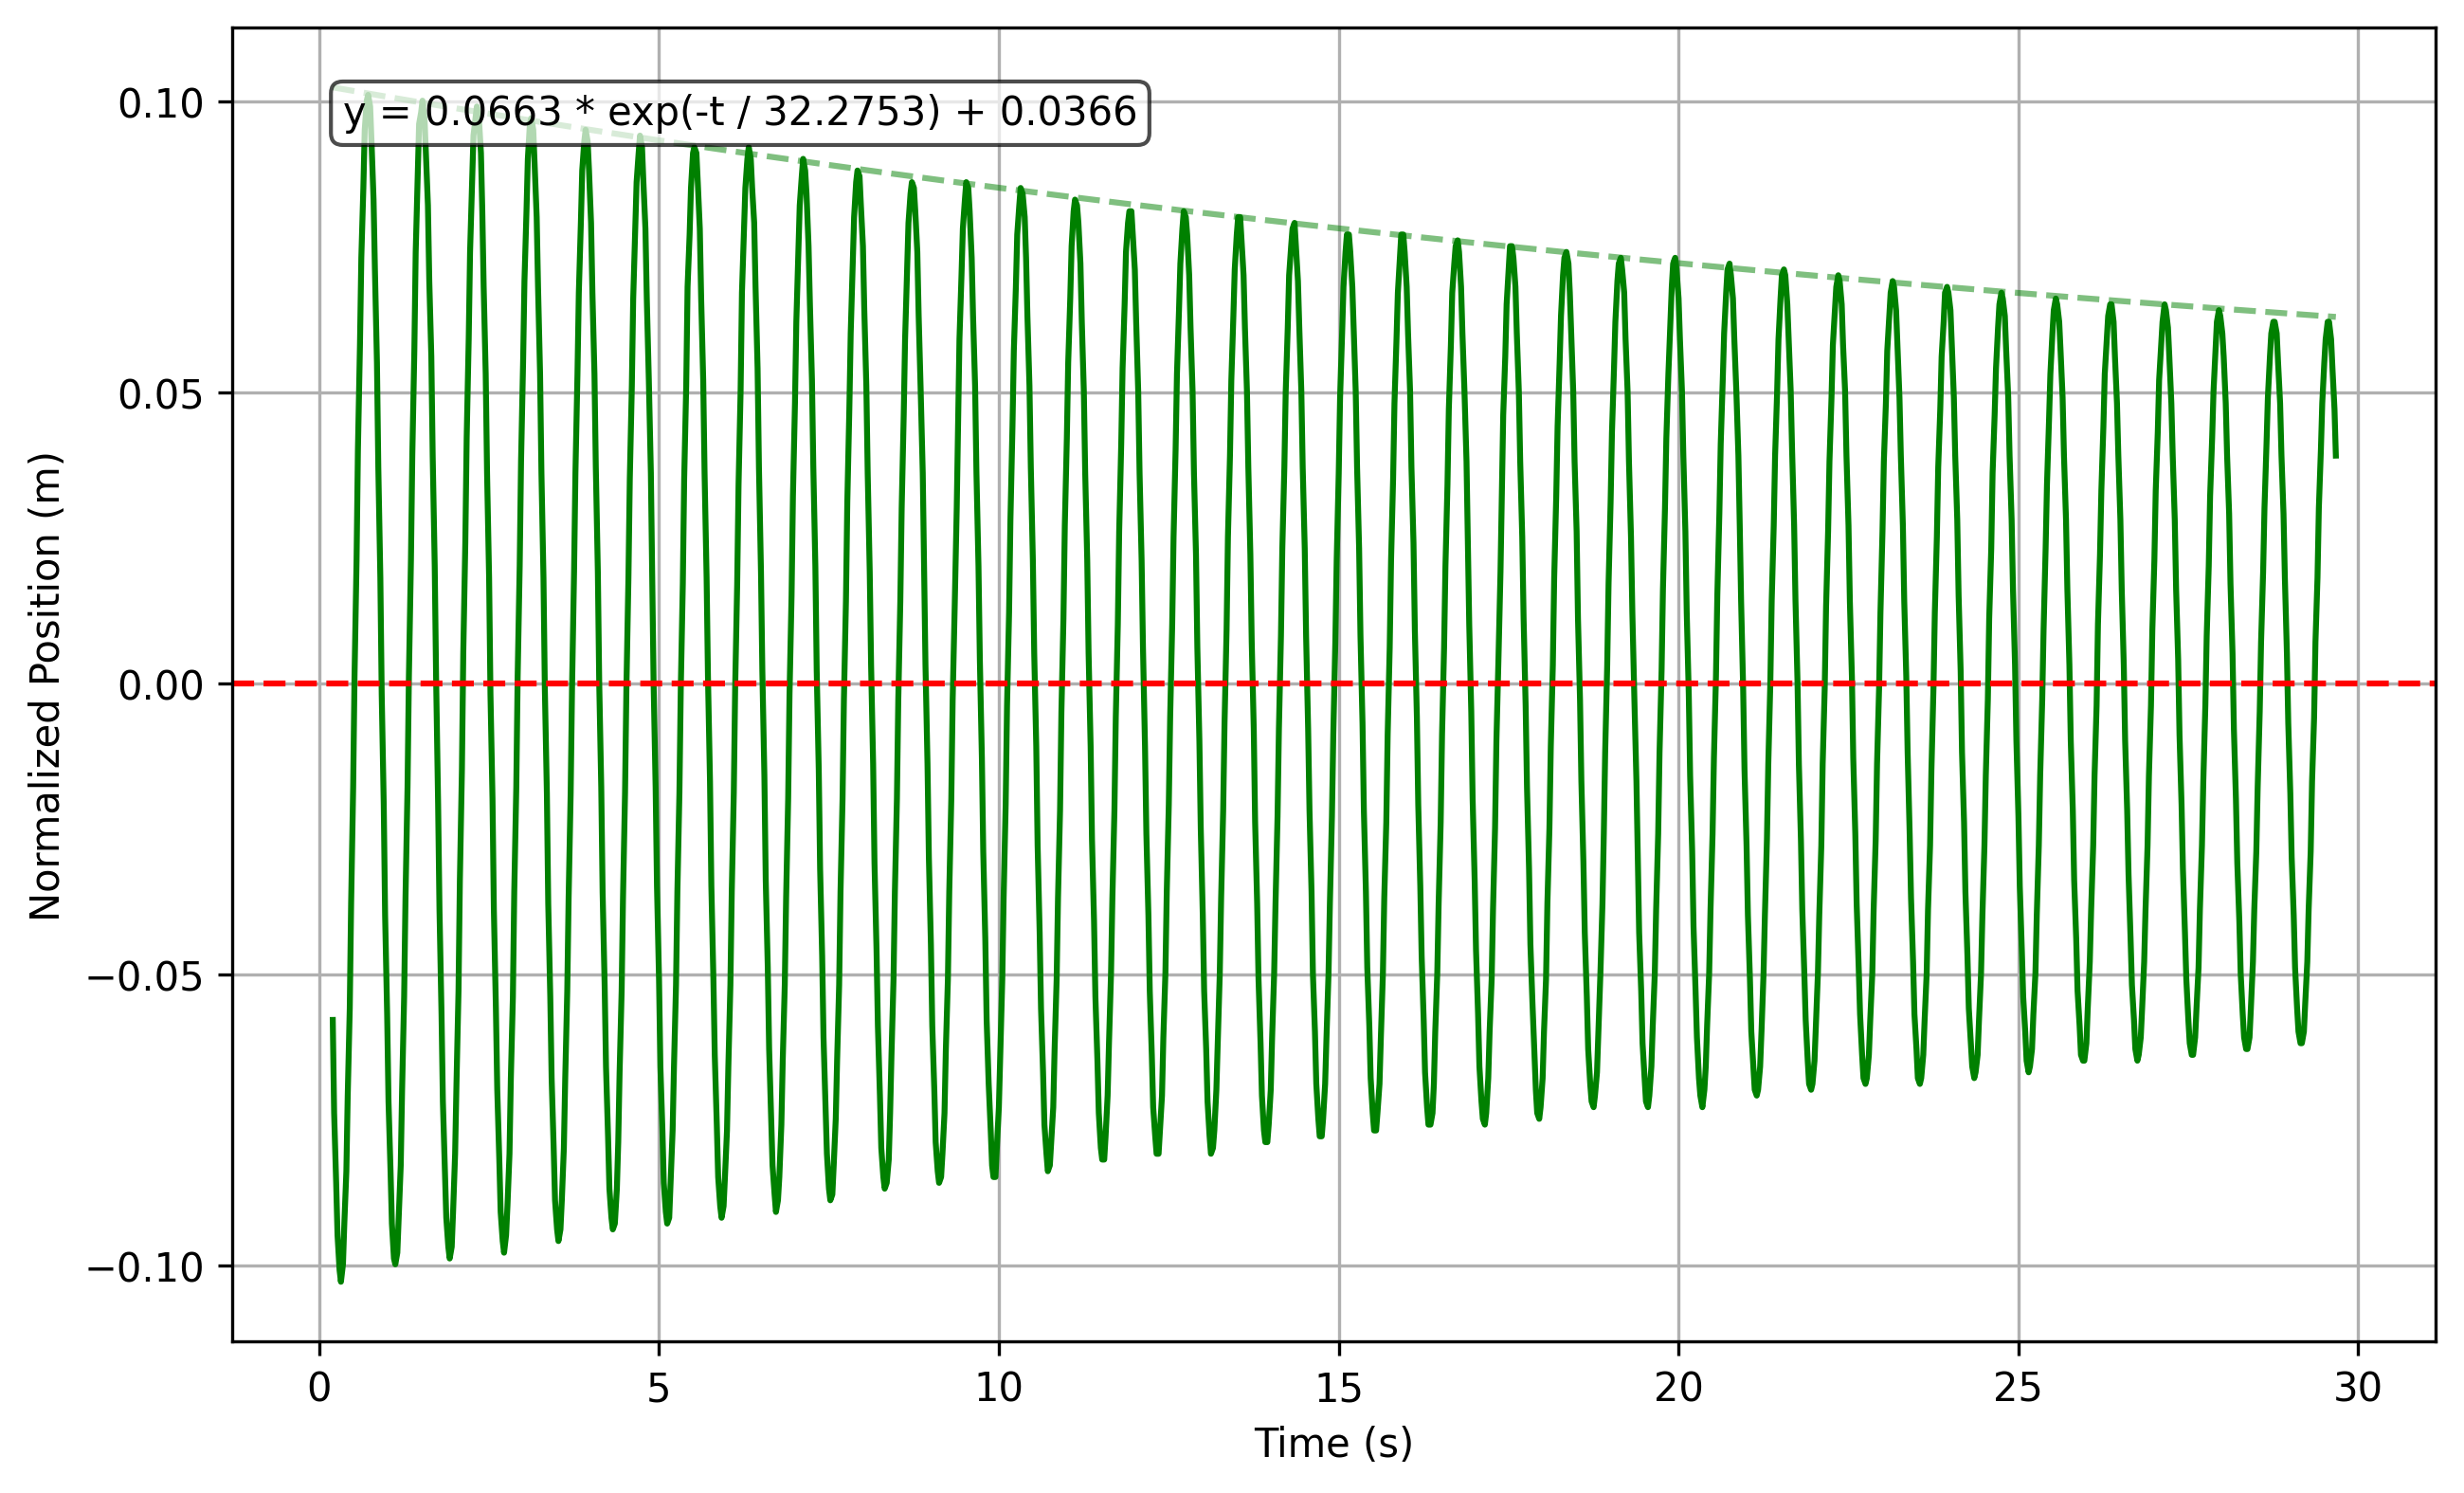
\includegraphics[width=\linewidth]{images/2cm.png}
  \caption{Spring with only 25g}\label{fig:2cm}
\endminipage\hfill
\minipage{0.5\textwidth}
  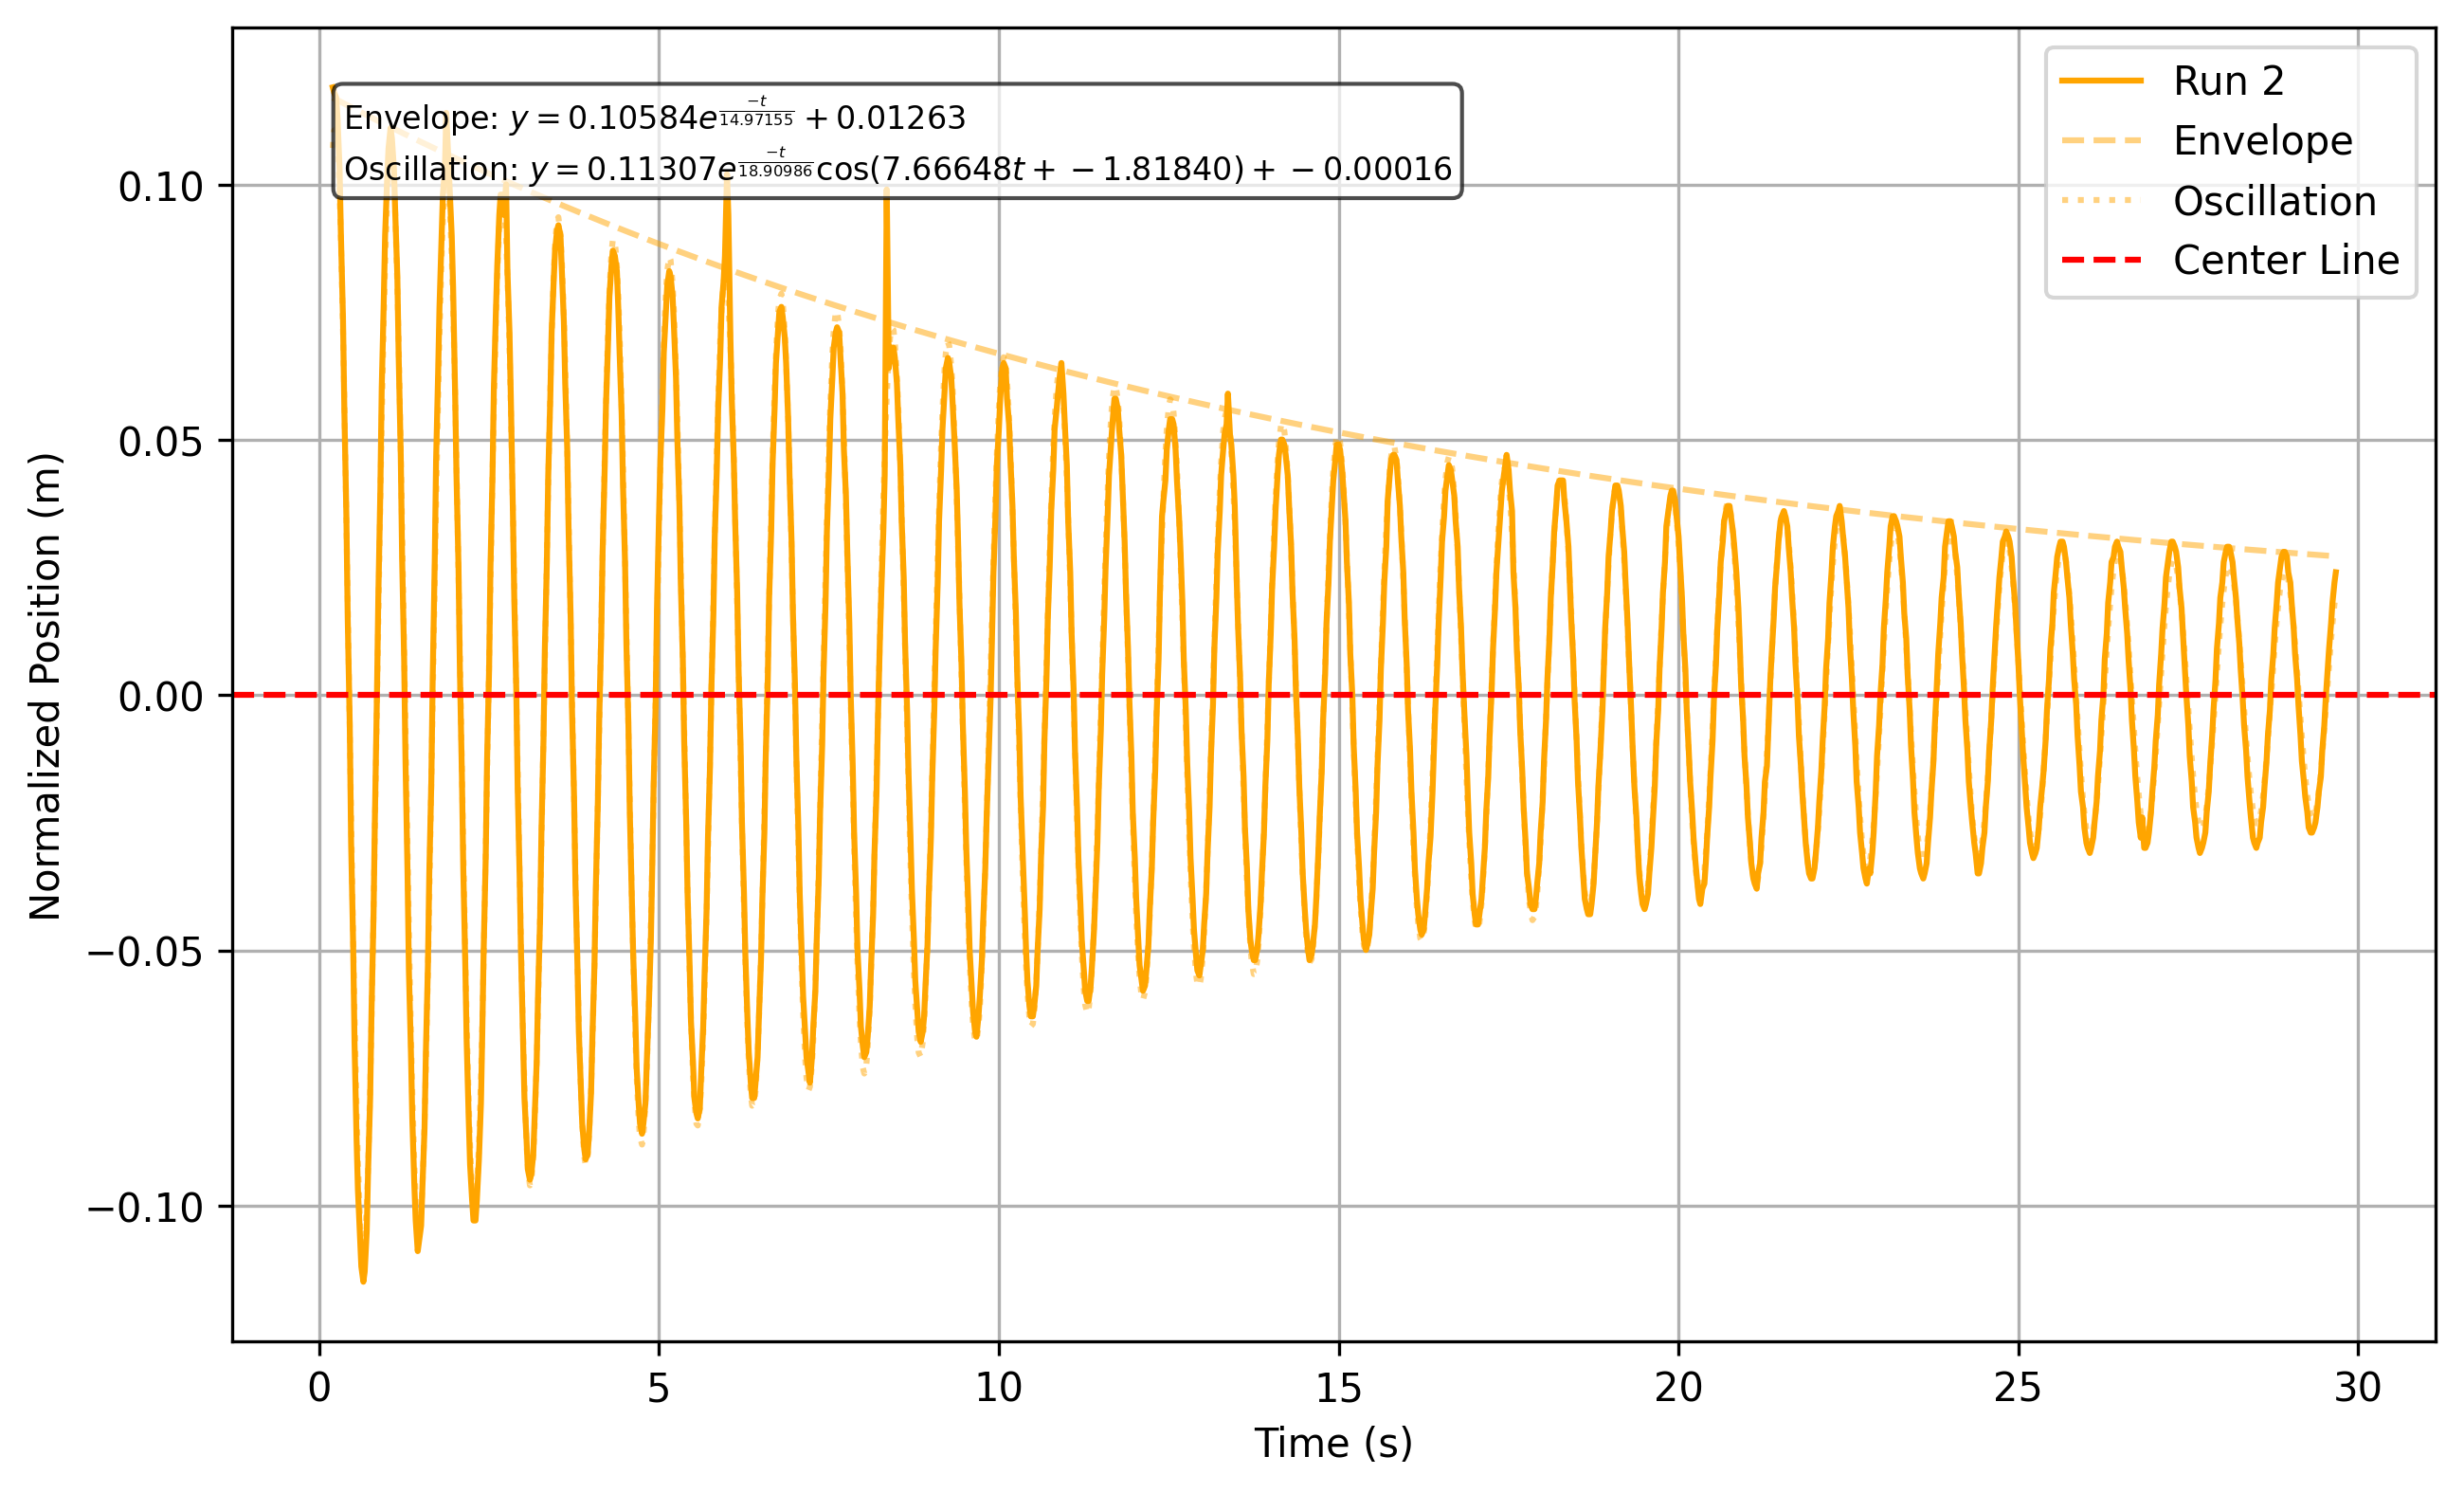
\includegraphics[width=\linewidth]{images/4cm.png}
  \caption{Spring with 25g and a 4cm disk}\label{fig:4cm}
\endminipage\hfill
\\
\minipage{0.5\textwidth}
  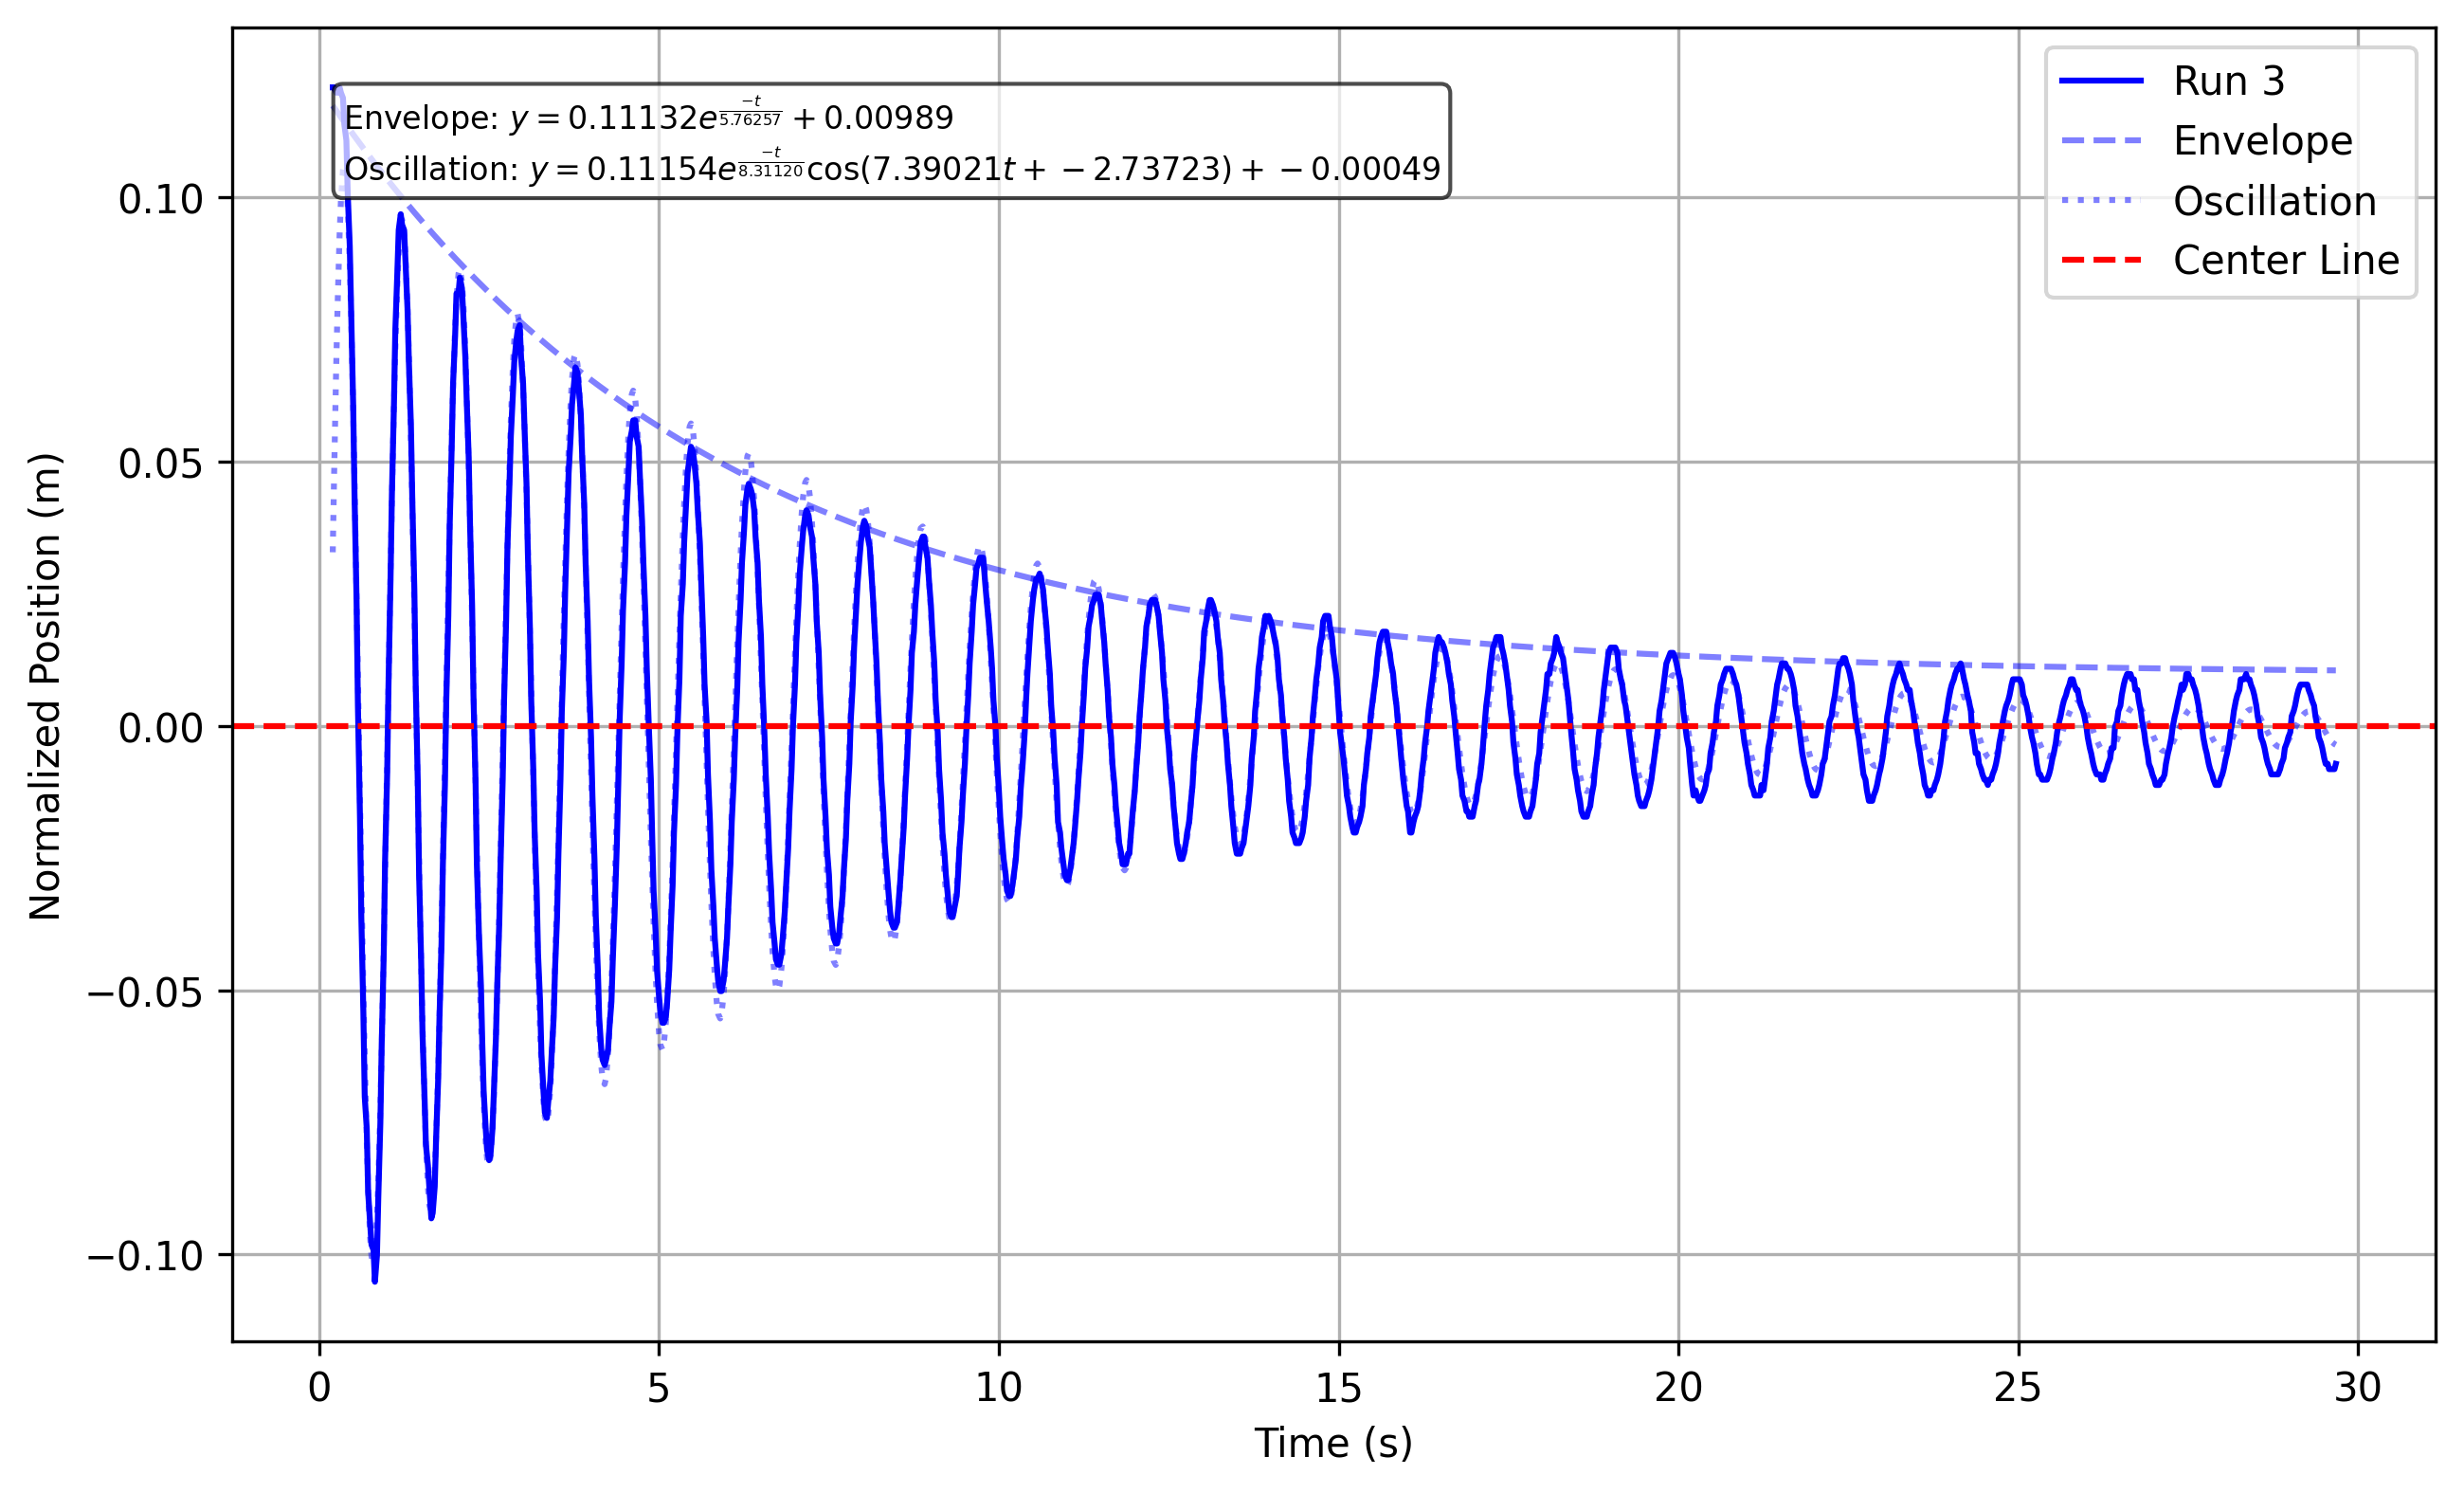
\includegraphics[width=\linewidth]{images/6cm.png}
  \caption{Spring with 25g and a 6cm disk}\label{fig:6cm}
\endminipage\hfill
\minipage{0.5\textwidth}
  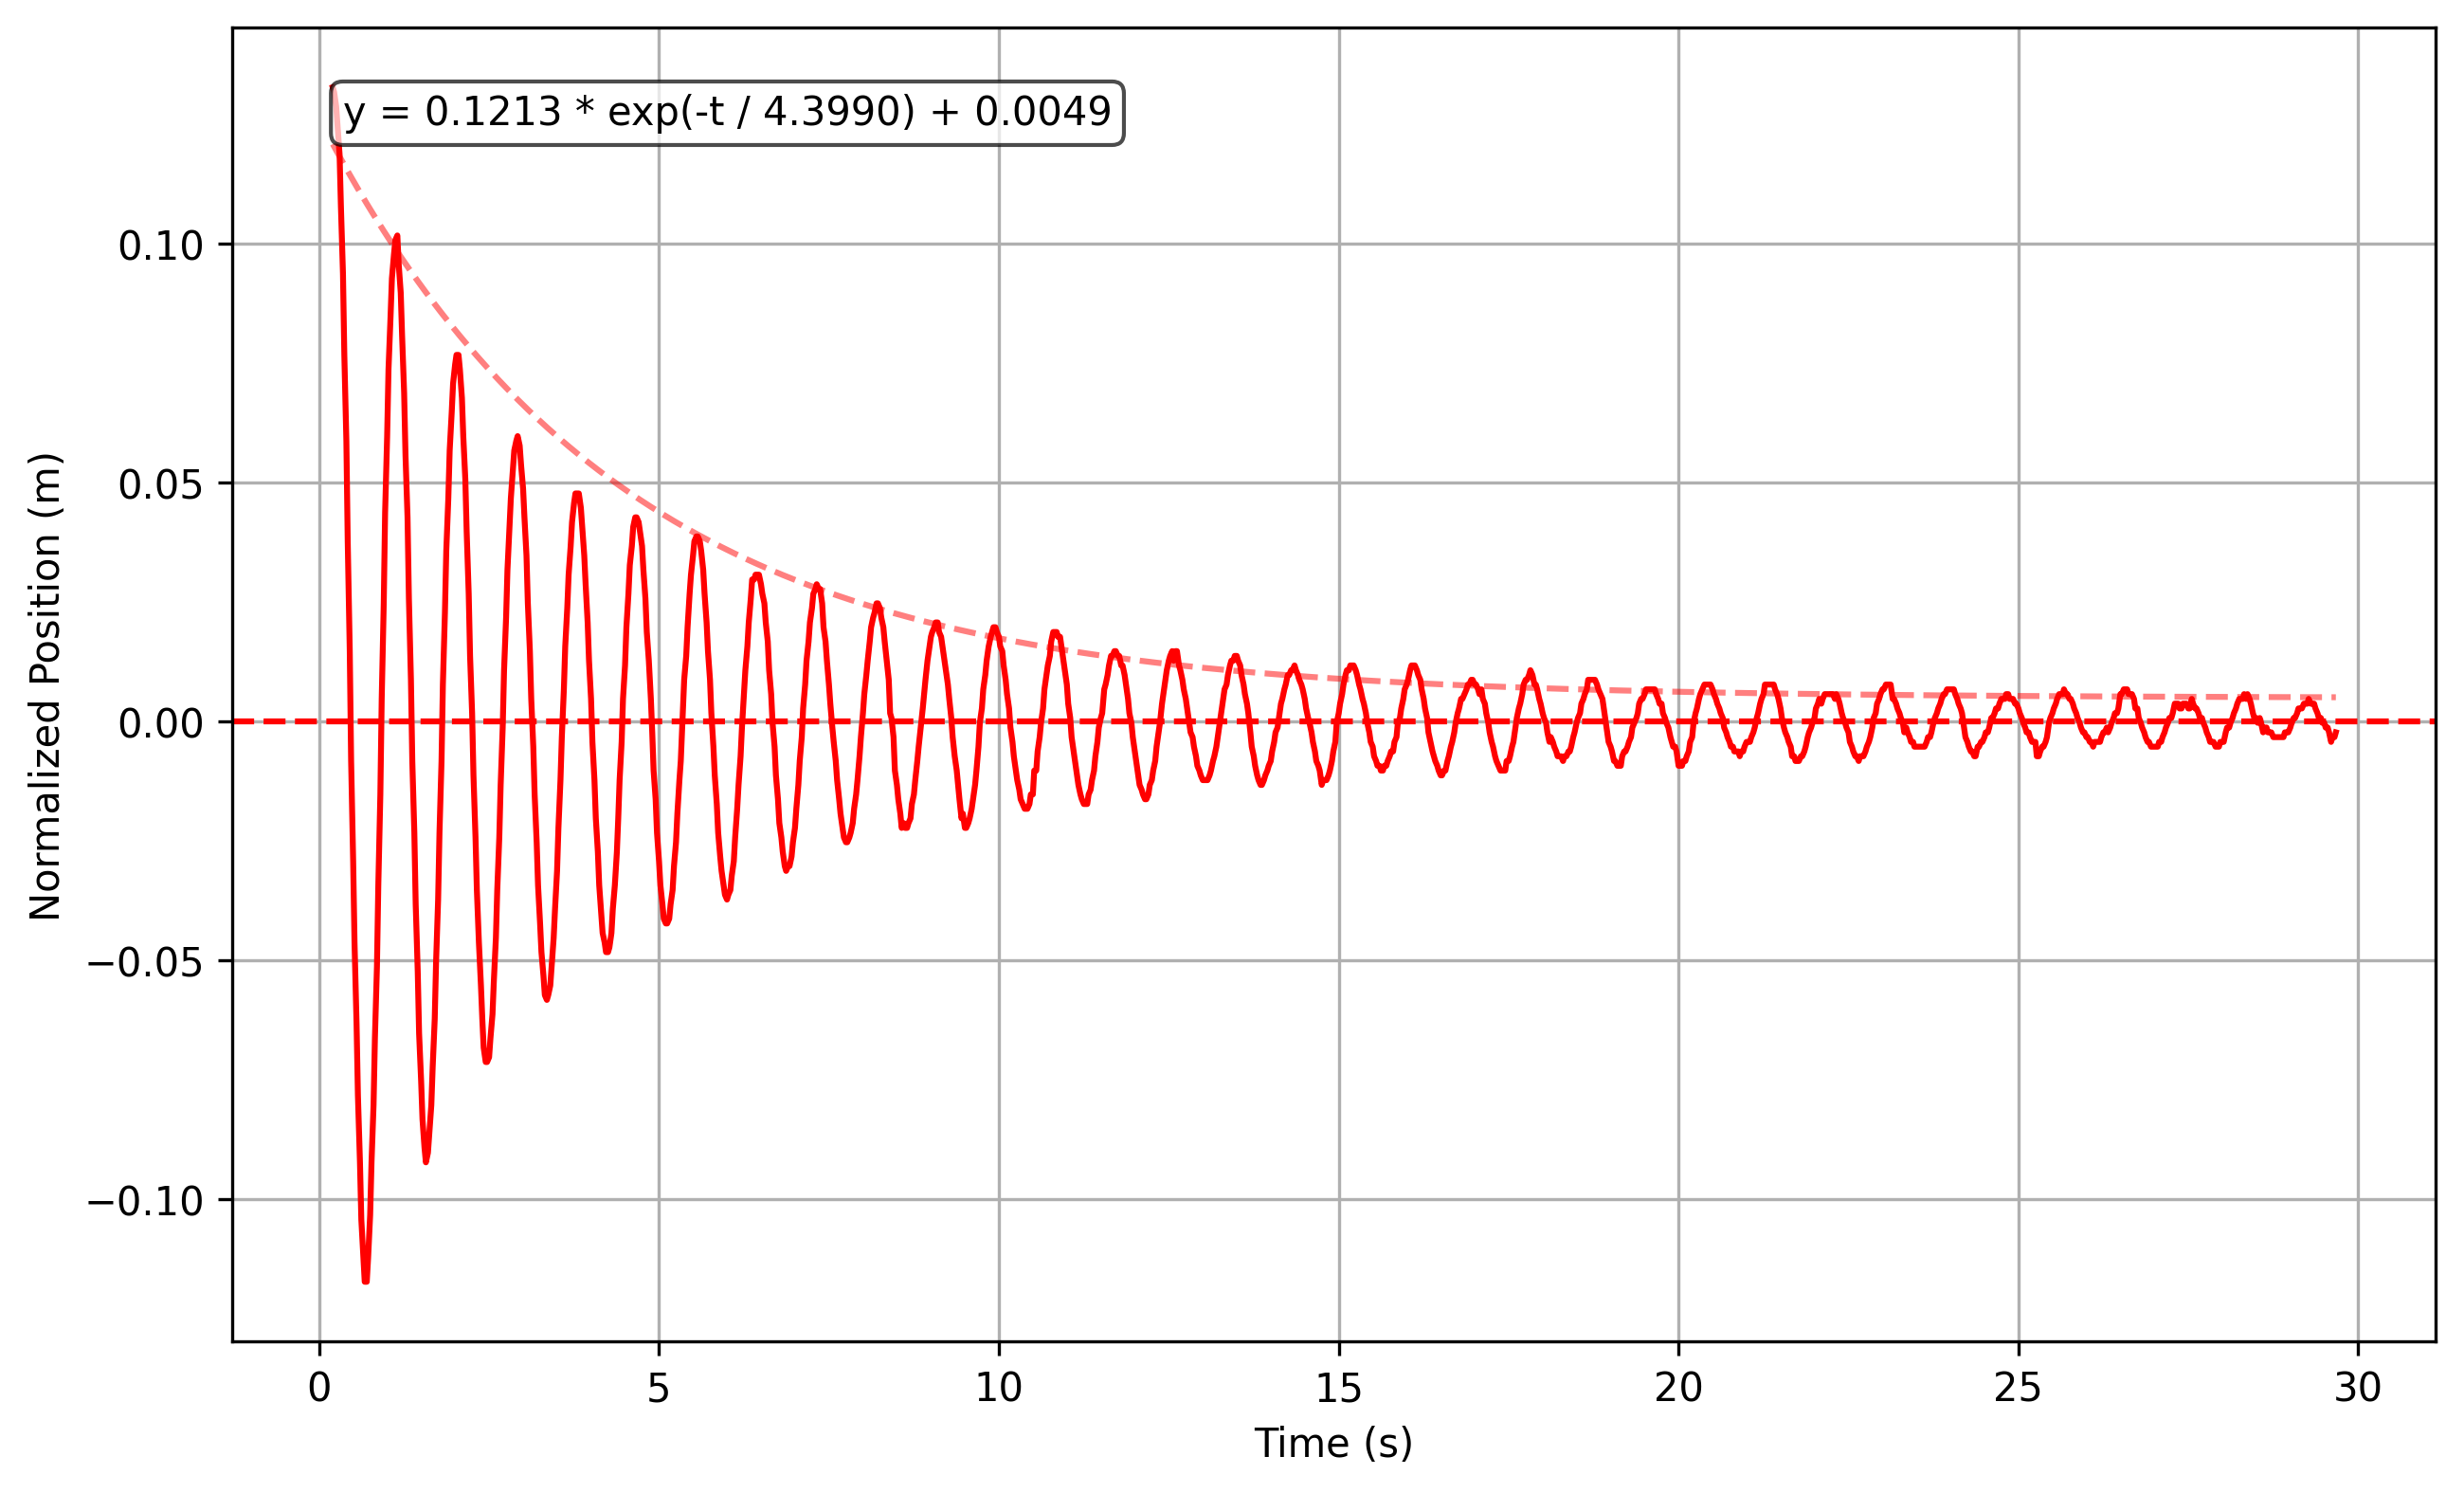
\includegraphics[width=\linewidth]{images/8cm.png}
  \caption{Spring with 25g and a 8cm disk}\label{fig:8cm}
\endminipage\hfill
\\
\minipage{0.5\textwidth}
  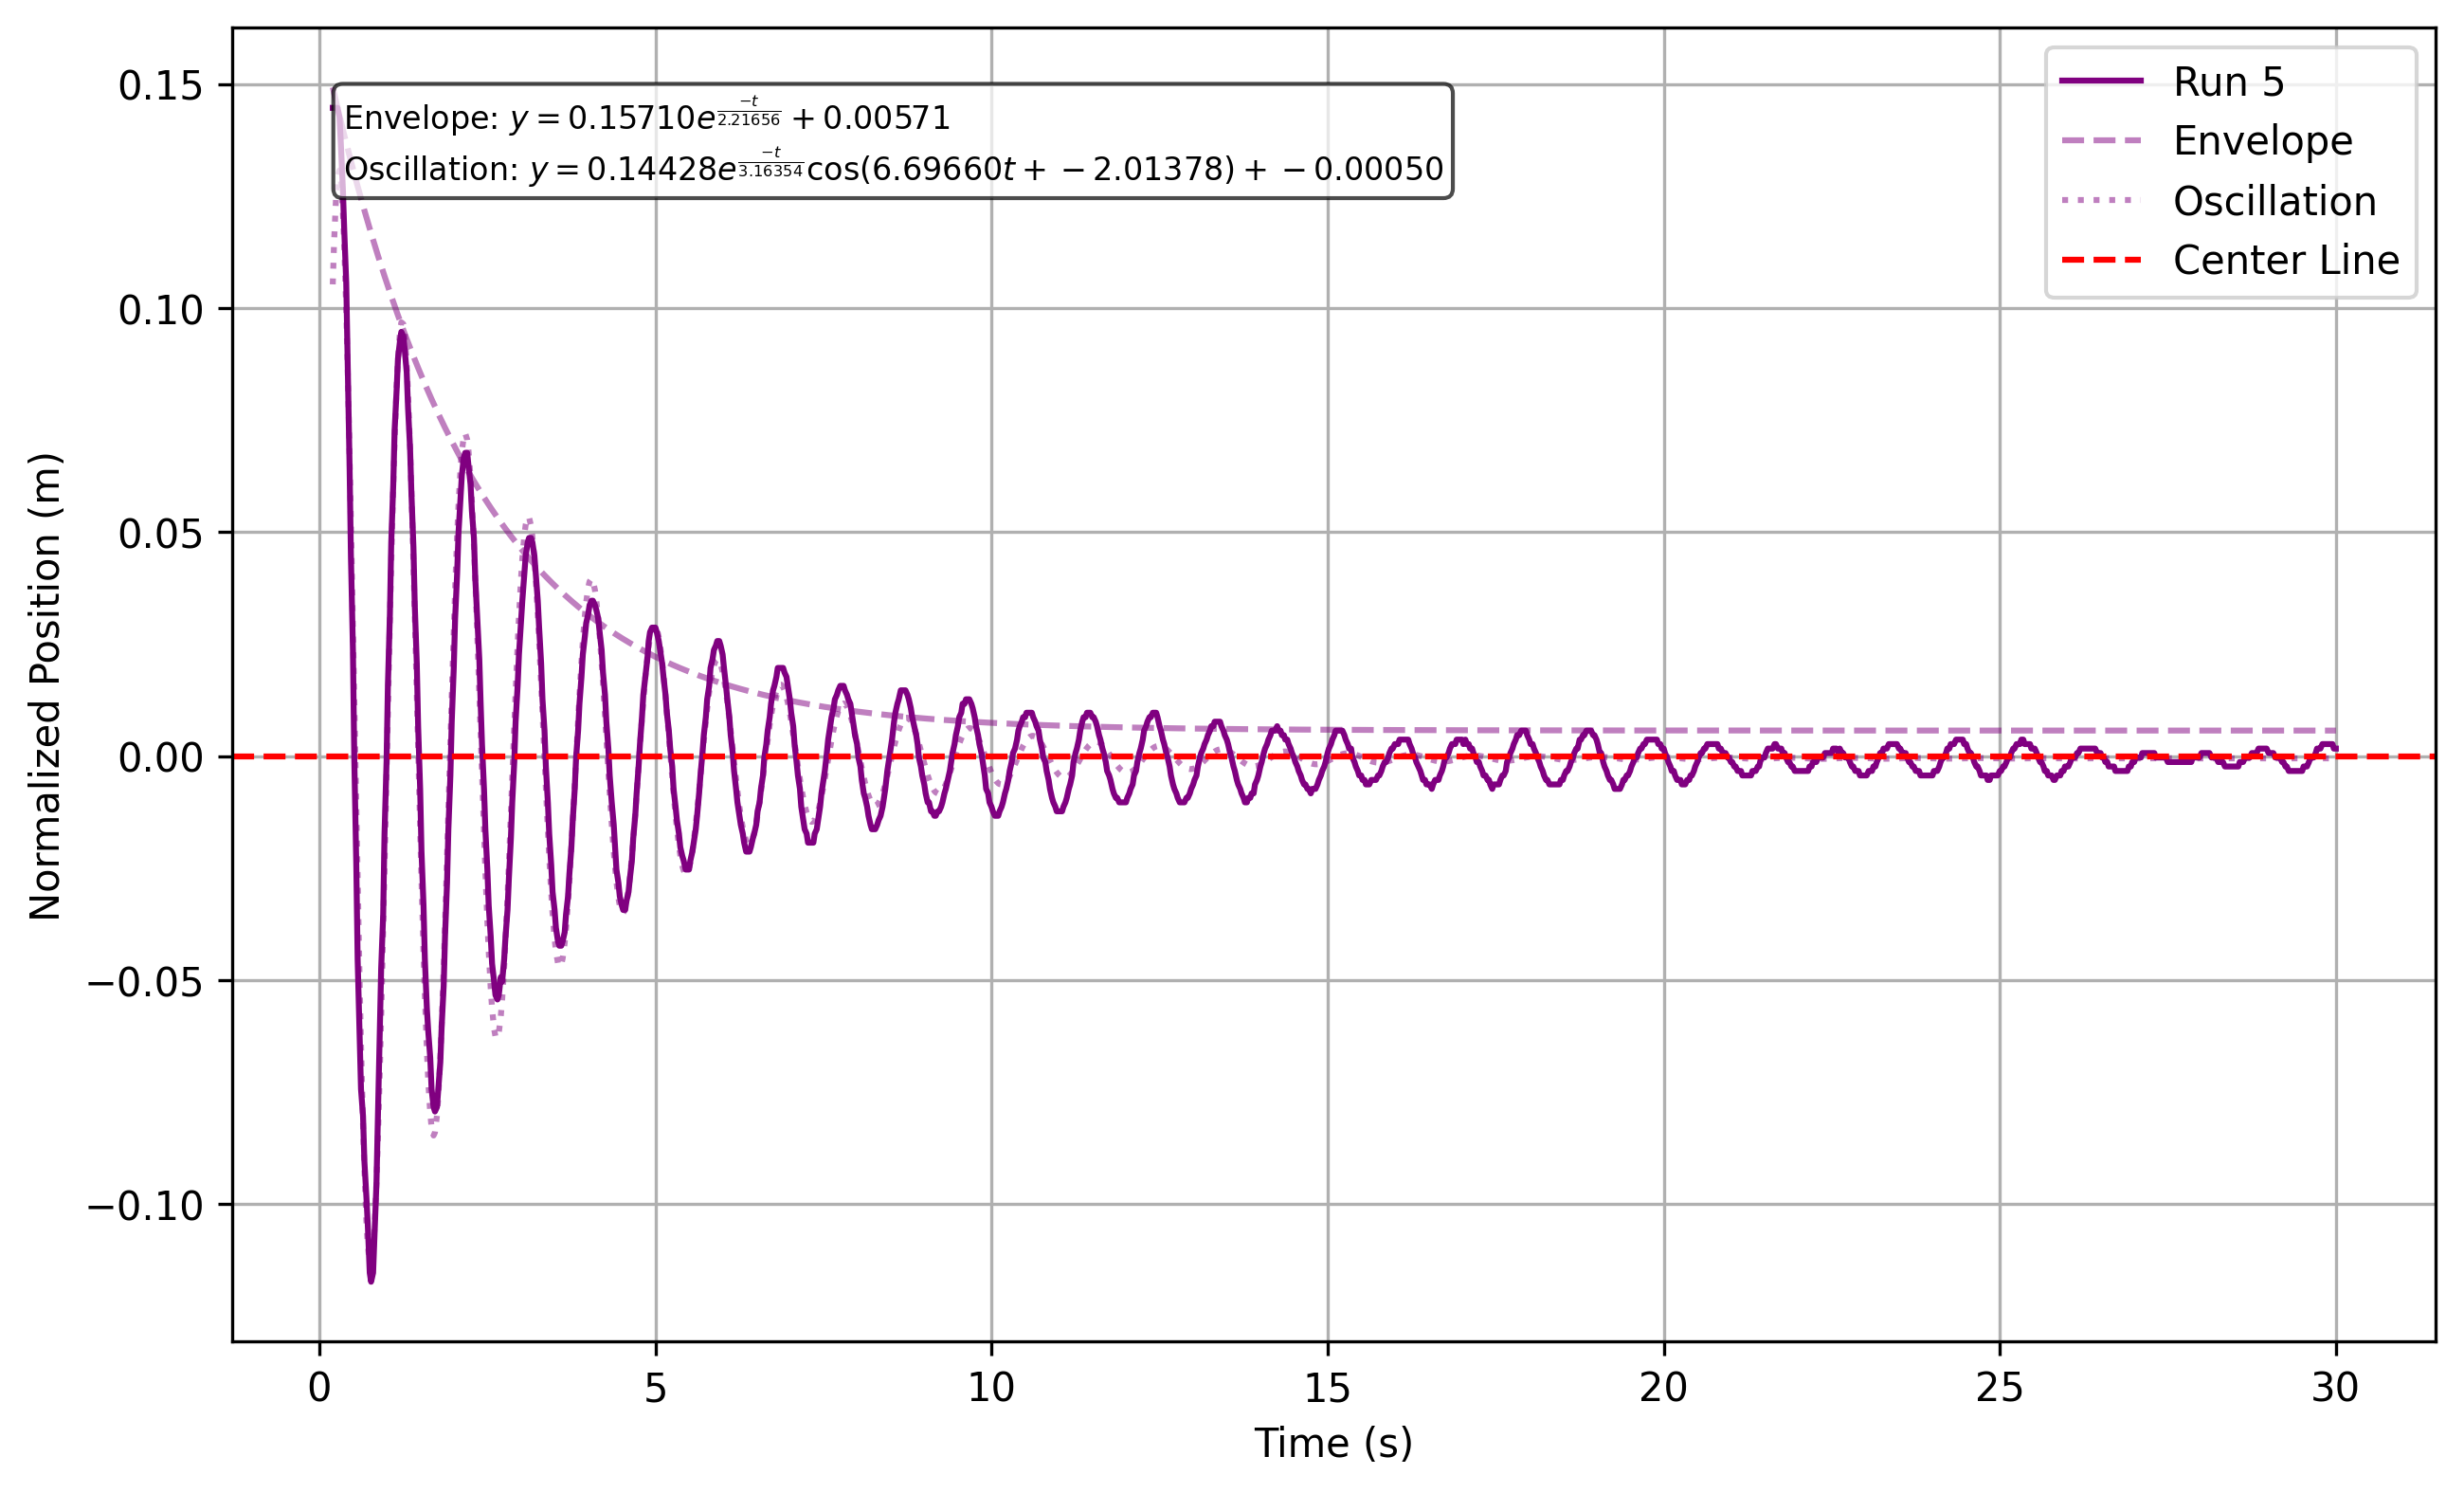
\includegraphics[width=\linewidth]{images/10cm.png}
  \caption{Spring with 25g and a 10cm disk}\label{fig:10cm}
\endminipage\hfill
\minipage{0.5\textwidth}
  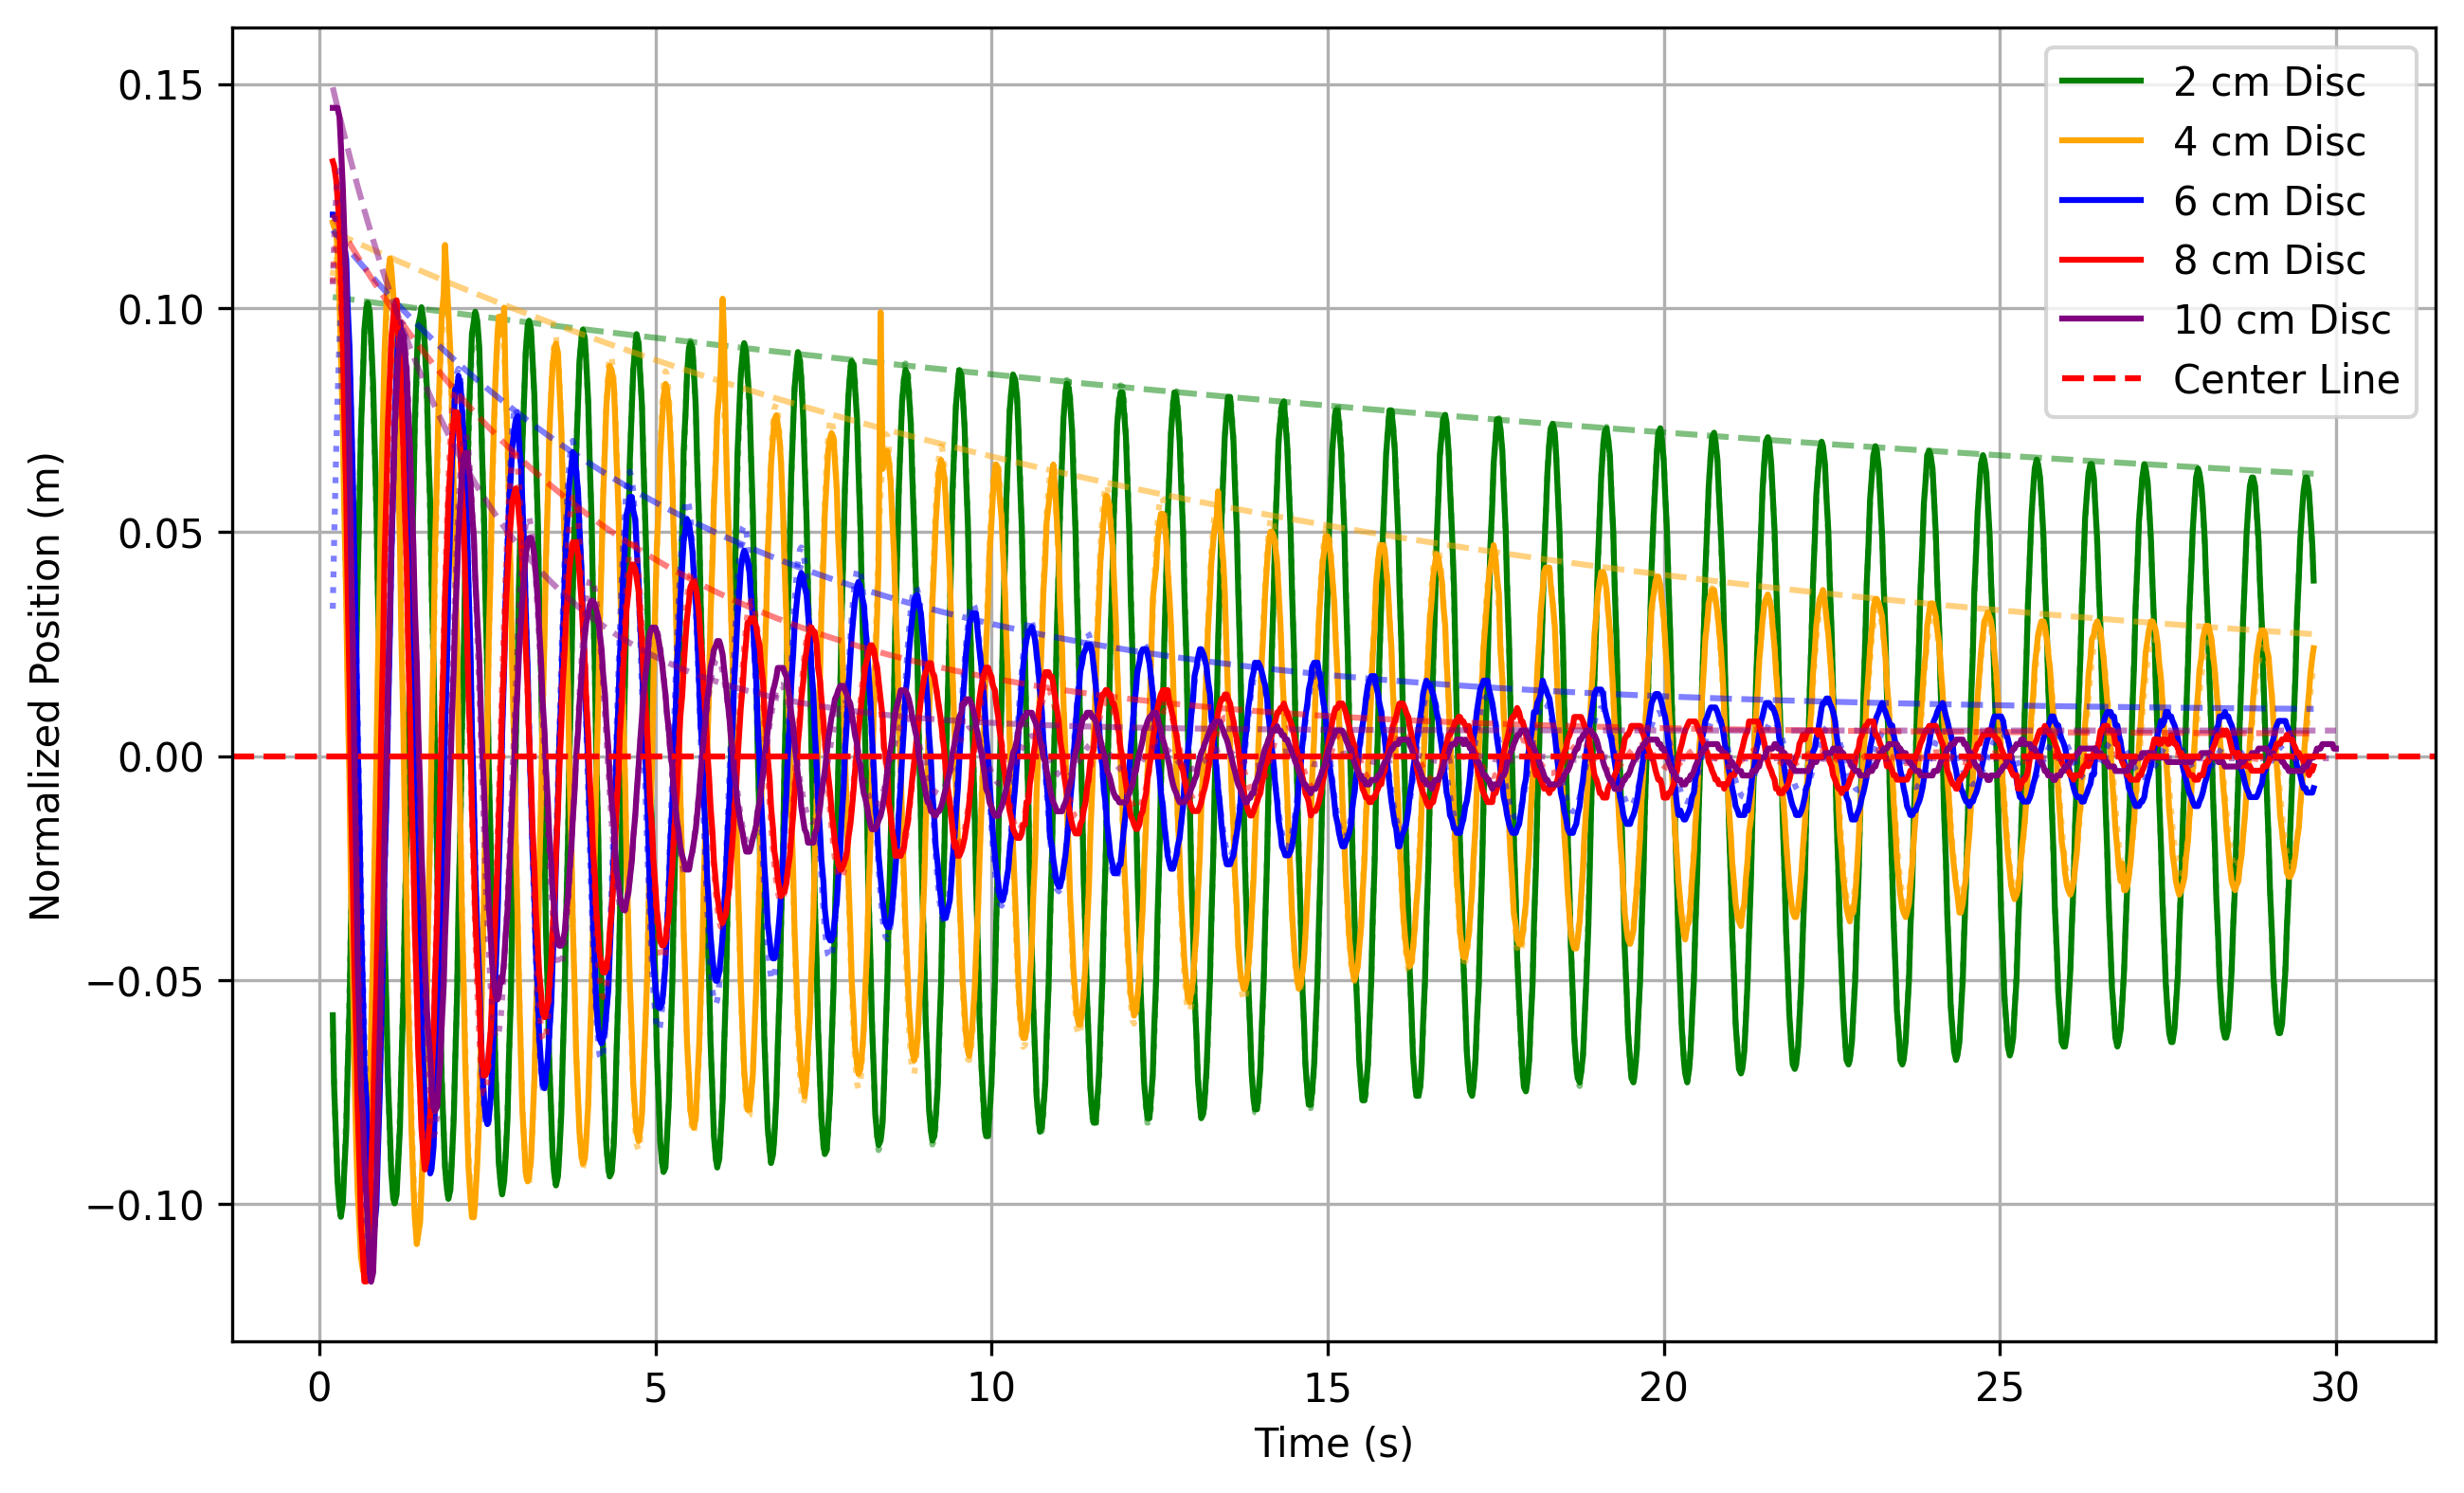
\includegraphics[width=\linewidth]{images/all.png}
  \caption{All oscillations overlaid}\label{fig:all}
\endminipage\hfill
\\
\minipage{0.5\textwidth}
  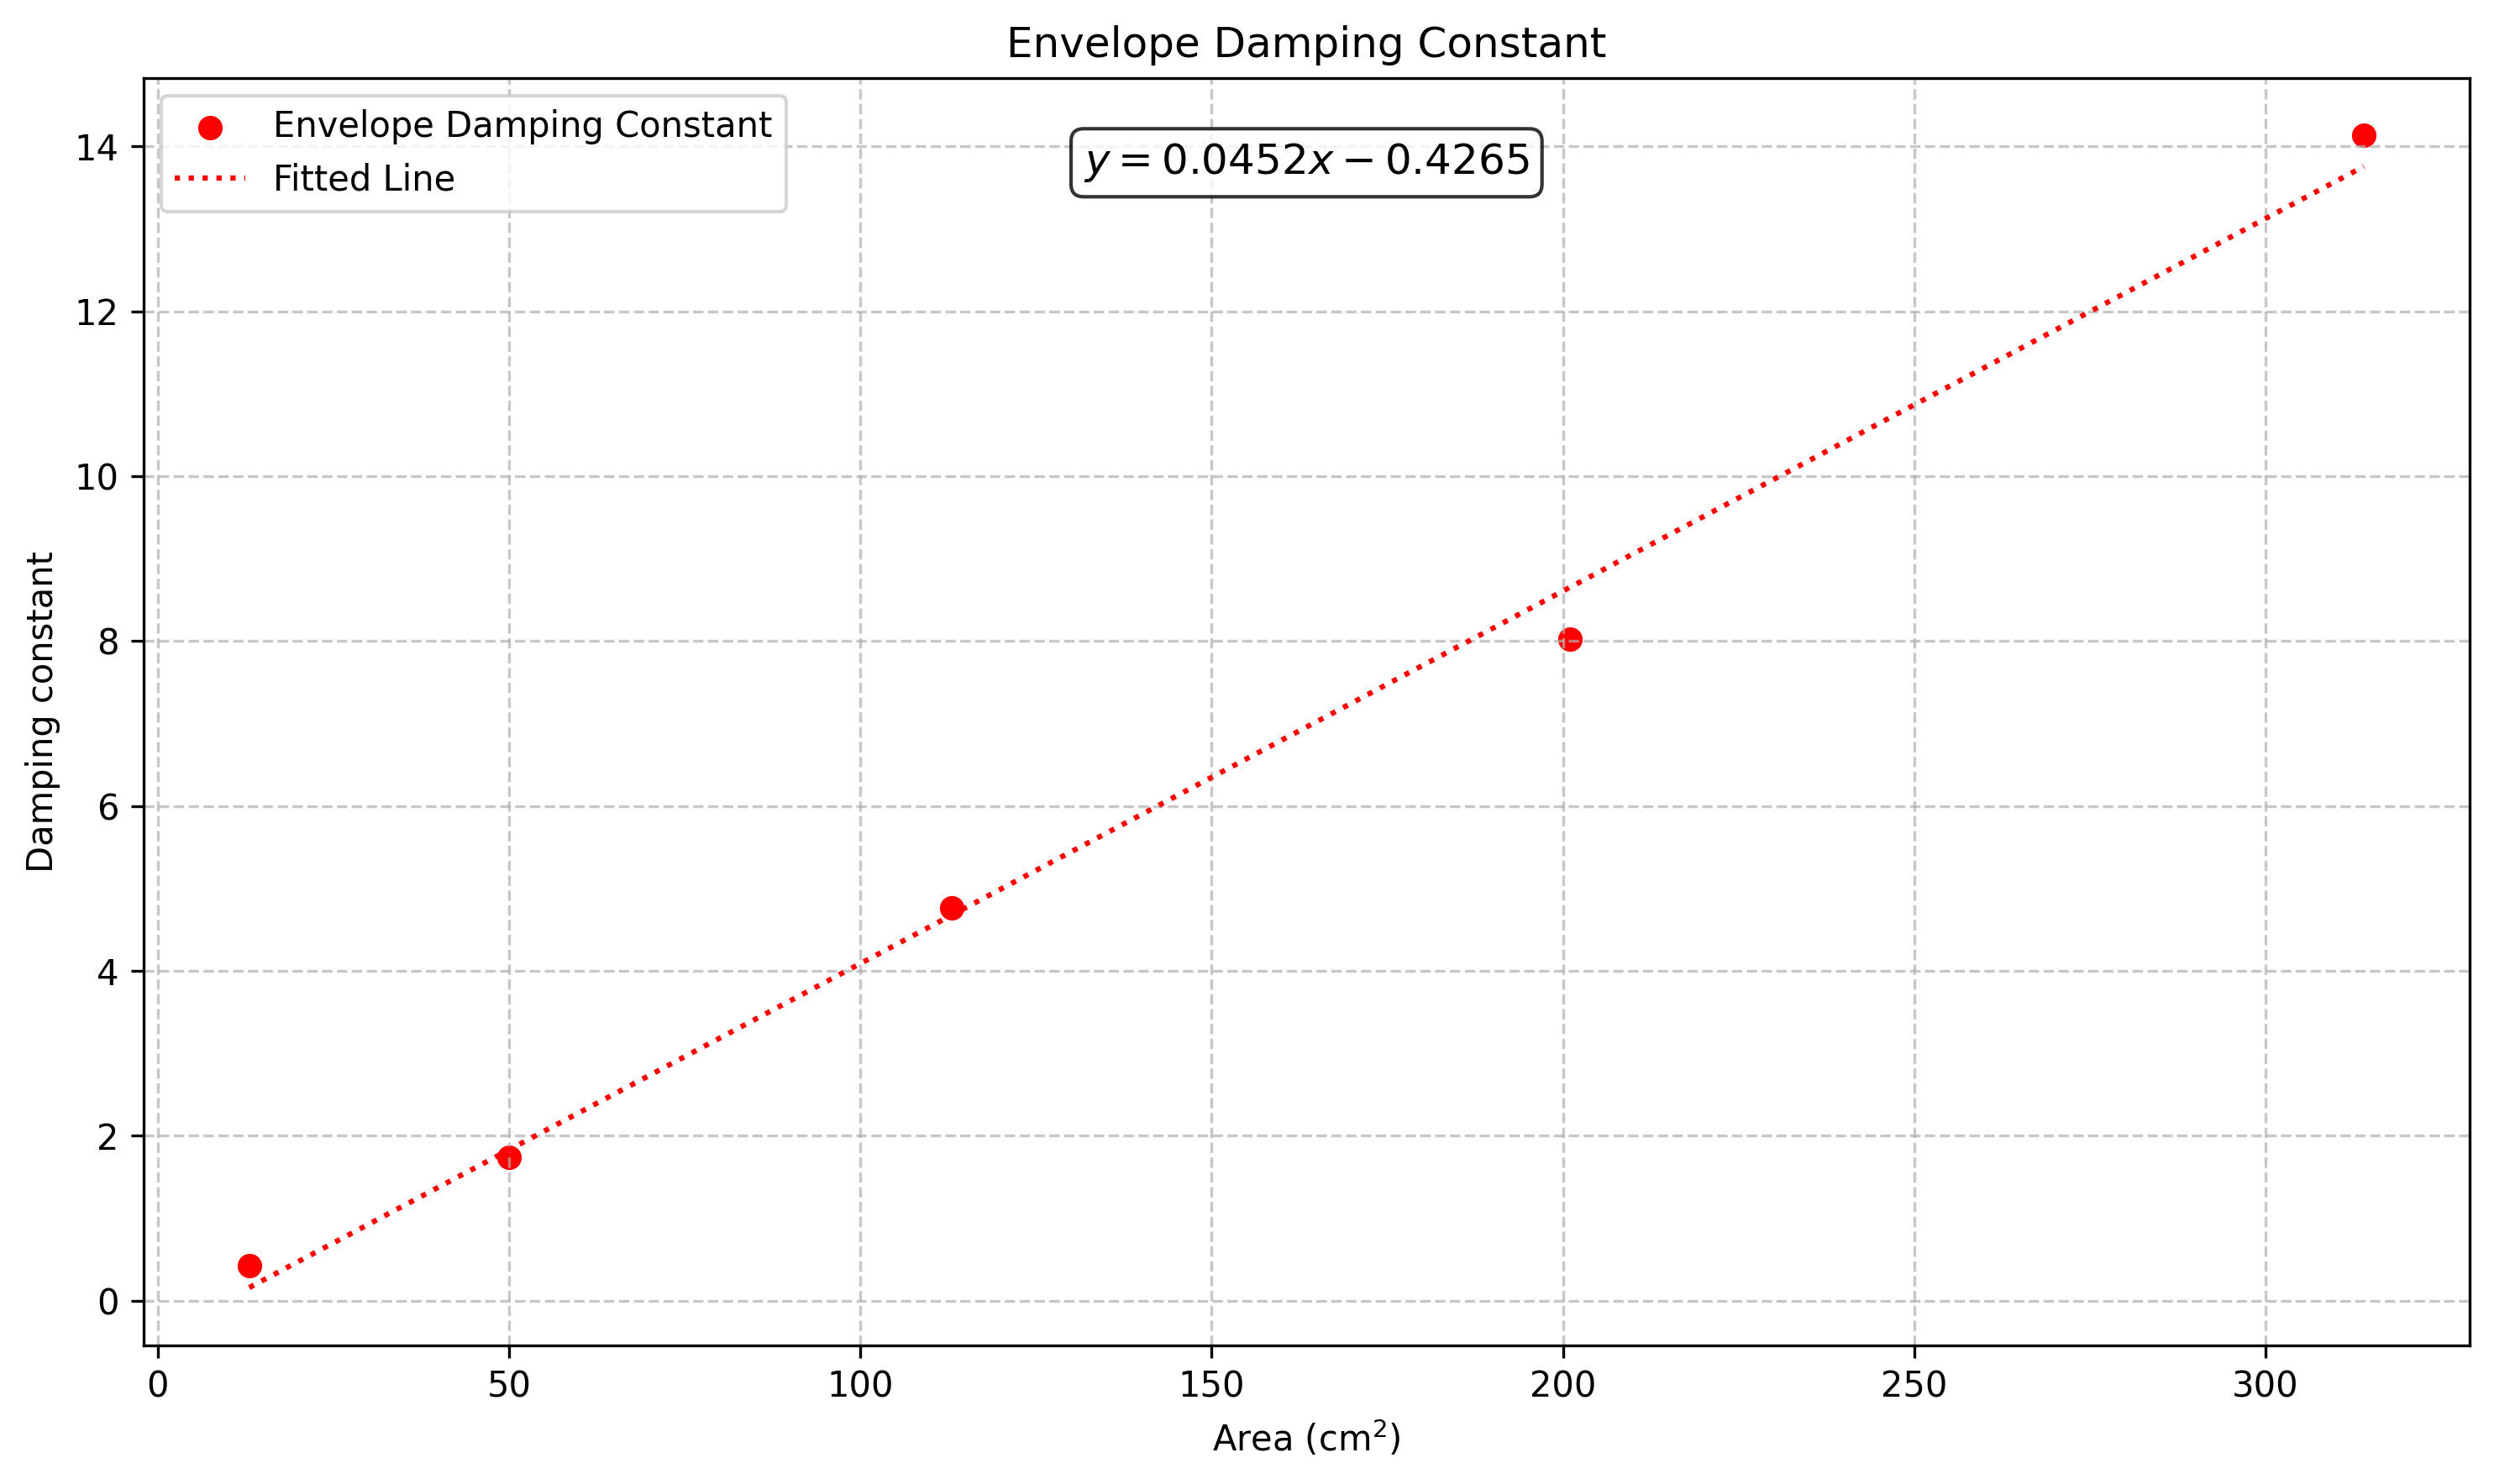
\includegraphics[width=\linewidth]{images/b-env.png}
  \caption{$b$ (from envelope) w.r.t. area}\label{fig:benv}
\endminipage\hfill
\minipage{0.5\textwidth}
  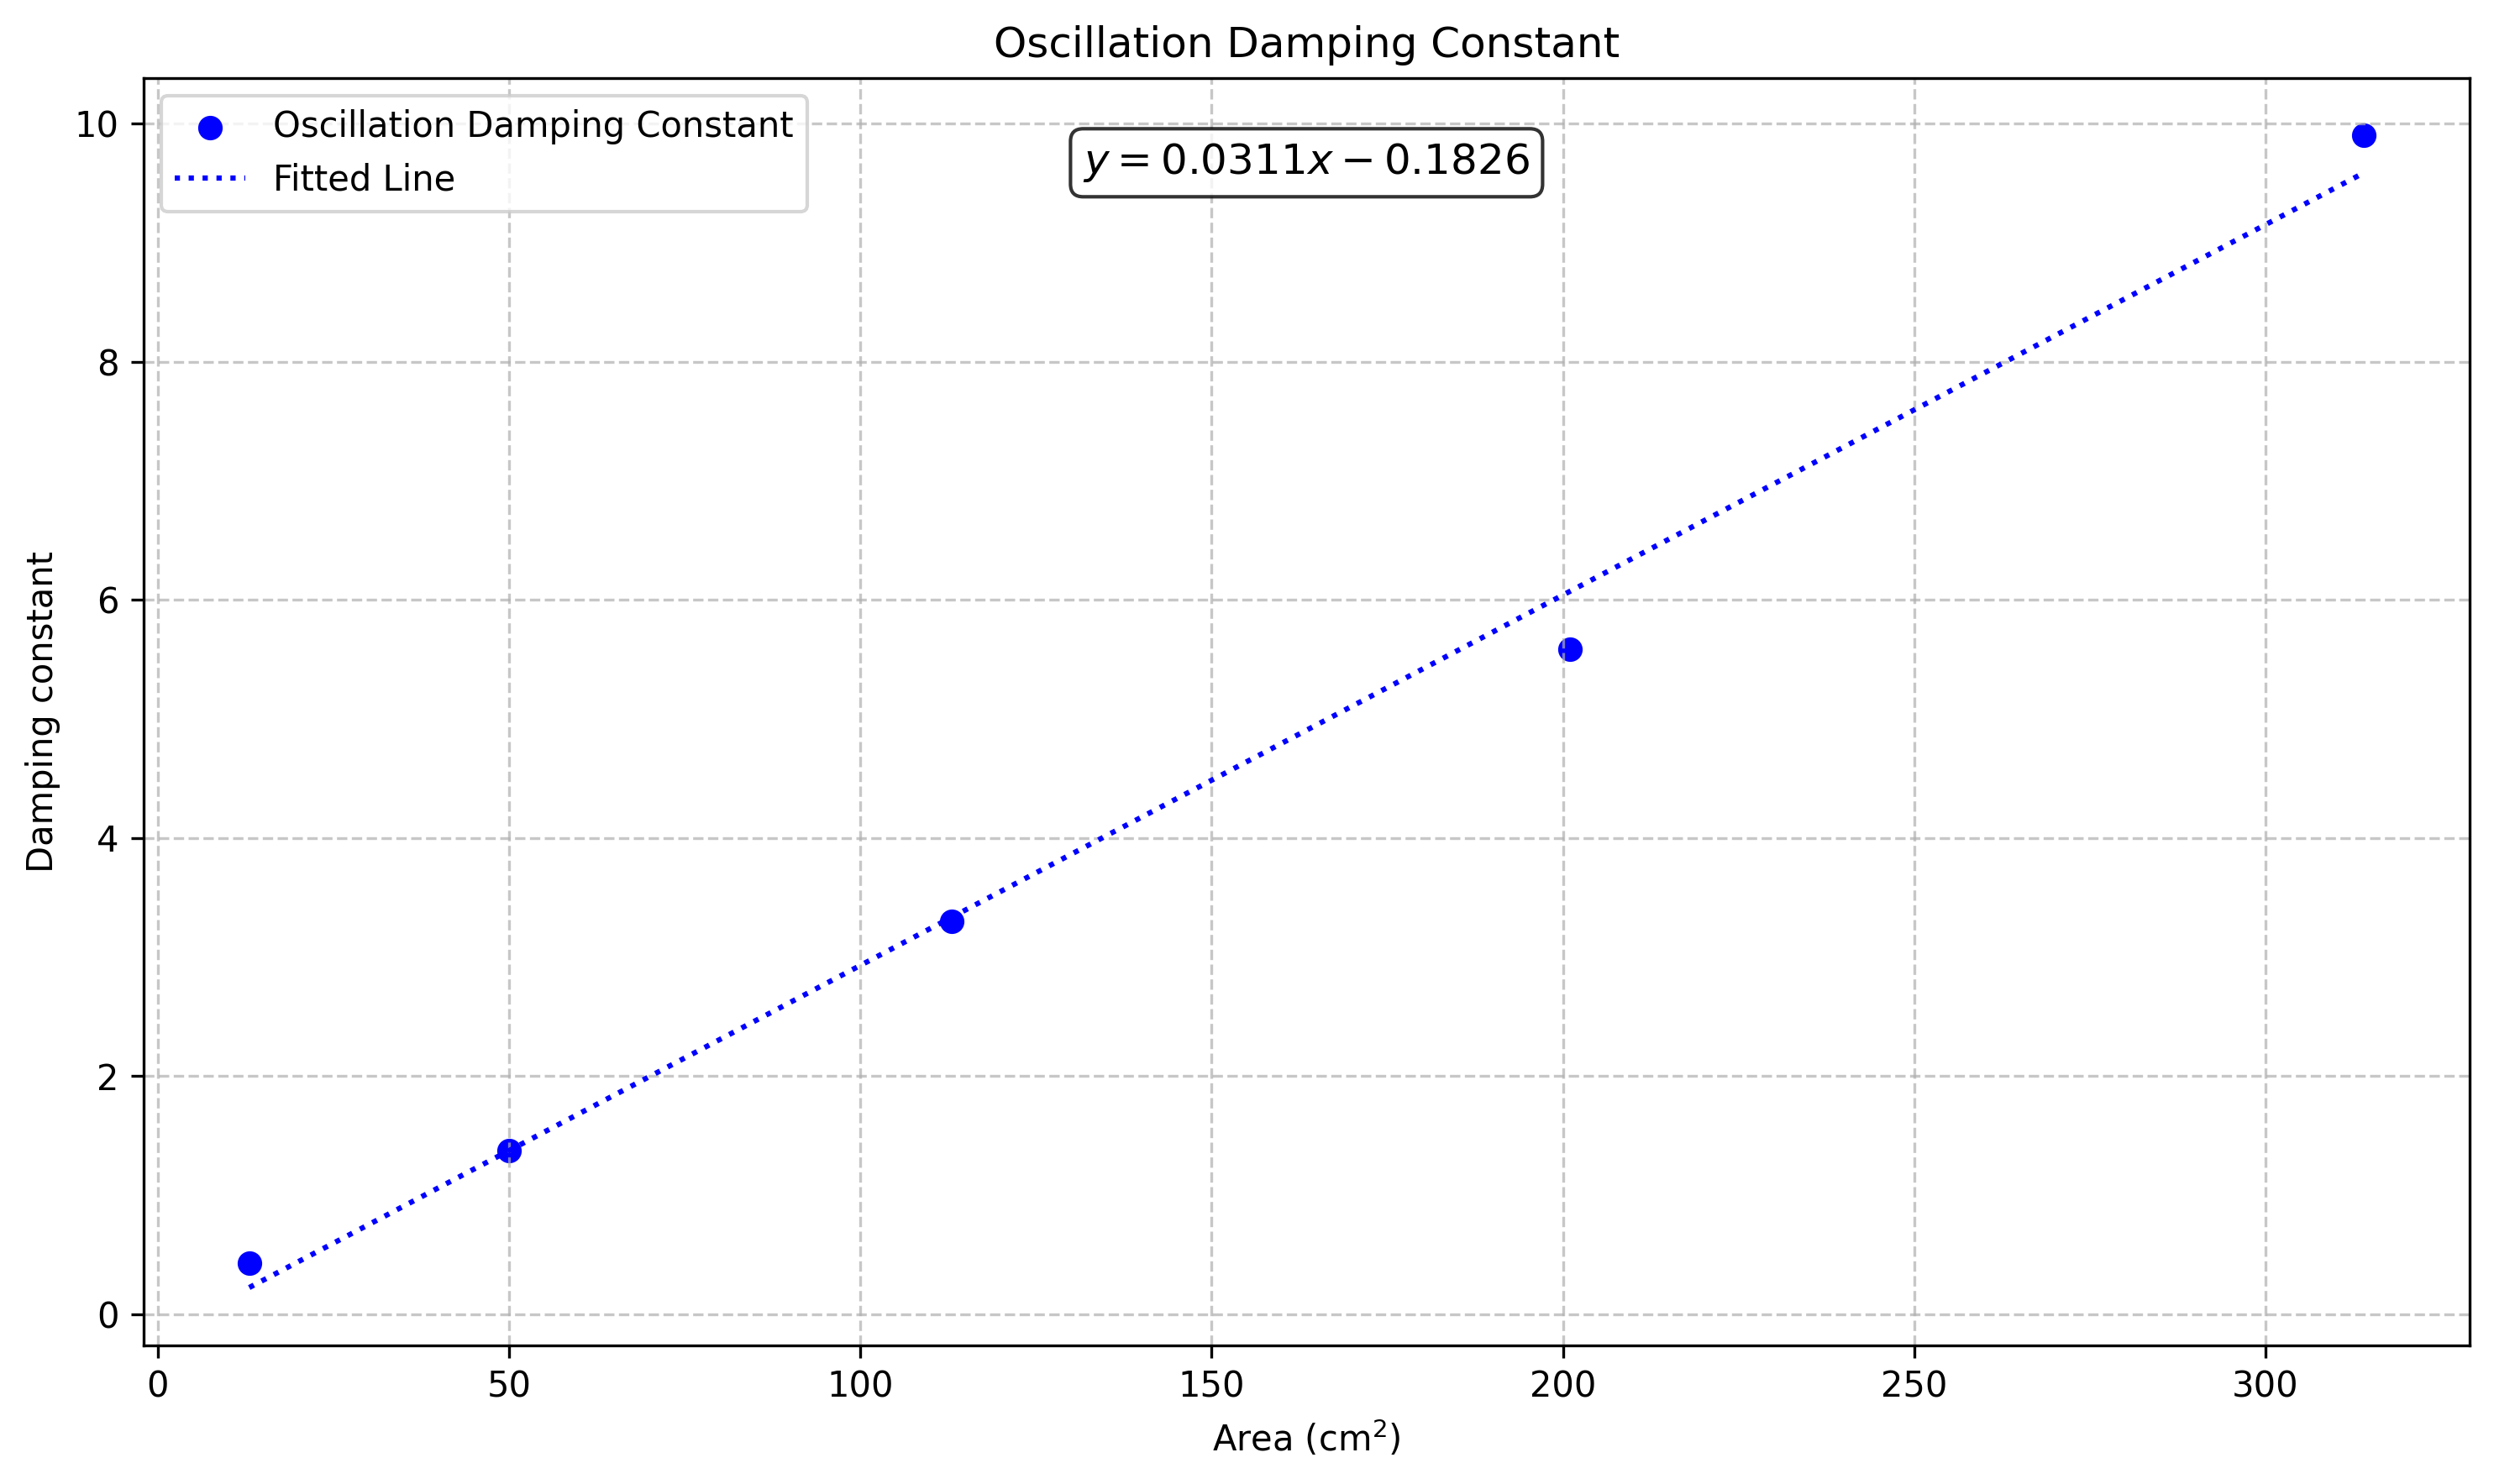
\includegraphics[width=\linewidth]{images/b-osc.png}
  \caption{$b$ (from oscillation) w.r.t. area}\label{fig:bosc}
\endminipage\hfill
\end{figure}


% \bibliographystyle{unsrtnat}
% \bibliography{references}

\end{document}
